%! Author = mariuszindel
%! Date = 24.01.21

\section{Responsive Design}

\textbf{Flexibles Layout:} Dynamisches Layout welches sich ohne Media-Queries umsetzen lässt\\
\textbf{Responsives Layout:} Dynamisches Layout welches für unterschiedliche Geräte separate Layouts definiert. Jedes Layout kann flexibel sein.\\
\textbf{Graceful Degradation} Eine Anwendung mit einer Basis an Funktionen in modernen Browsern erstellt wird und dann die Schichten entfernt werden, um sicherzustellen, dass sie mit älteren Browsern funktioniert\\
\textbf{Progressive Enhancement} Gegenteil von Graceful Degradation.\\
\textbf{Mobile First (vs. Desktop First)} Ähnlich wie Progressive Enhancement


\subsection{Responsive Web layout}
\subsubsection{Media Queries}
\begin{lstlisting}
// Typen
@media screen { ... }
@media print { ... }
// Dimensionen
@media ( [ width | min-width | max-width ] : 375px) { ... }
@media ( [ height | min-height | max-height ] : 667px) { ... }
//Zustaende
@media (orientation: landscape) { ... }
//Features
@supports not (display: grid){div {float: right;}}
//Sonstiges
@media (hover: hover) { ... }
@media (min-resolution: 300dpi) { ... }
// Operatoren
@media (min-width: 20em) and (max-width: 30em) {}
@media not screen {...}
@media not screen and (min-width: 20em) {...}
\end{lstlisting}
Link Referenzen mit Media-Attribut nur wenn erfüllt
\begin{lstlisting}
<link rel="stylesheet" href="LargeScreenLayout.css" media="(min-width: 30em)">
\end{lstlisting}

\subsubsection{Viewport}
Mobile Geräte benötigen Viewport Meta-Tag Spezifikation, damit die Media-Query ''greift''.
\begin{lstlisting}
<meta name="viewport" content="width=device-width,initial-scale=1">
\end{lstlisting}


\subsection{Flexibles Layout}

\subsubsection{CSS Box Layout}
\begin{minipage}{0.7\linewidth}
\begin{center}
    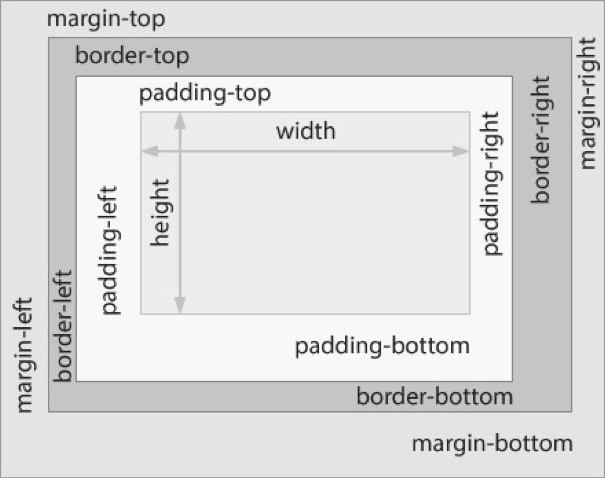
\includegraphics[width=\linewidth]{graphic/responsive/boxmodel.png}
\vspace{-8pt}
\end{center}
\end{minipage}
\begin{minipage}{0.287\linewidth}
    Box-Sizing Model gilt nur, wenn display: block oder inline-block aktiv\\
    Zentrieren von Elementen: \texttt{max-width: 50em; margin 0 auto;}
\end{minipage}
\textcolor{subsectioncolor}{CSS Funktionen}
\begin{lstlisting}
width: calc(100vw - 5em); //100vw = 100% ViewWidth
width: min(500px, 100vW - 5em);
width: max(400px, 100vw - 5em);
width: clamp(400px, 100vw - 5em, 500px);
//untere Grenze, Bevorzugt, obere Grenze
\end{lstlisting}
\textcolor{subsectioncolor}{Werte von Position}
\begin{itemize}
    \item \textbf{absolute} Element aus dem Element-Fluss entfernt $\rightarrow$ Erlaubt Überlappung von Elementen \\
    top, left, bottom, right, width, height
    \item \textbf{fixed} Element fix an einem Ort
    \item \textbf{sticky} Mischung zwischen absolut und fixed
    \item \textbf{relative} Referenz für Kind-Elemente welche mit position: absolut positioniert
    \item \textbf{static} Default Wert -> Element ist im Fluss
\end{itemize}


\subsubsection{Flexbox}
\begin{itemize}
    \item display: flex
    \item Betrifft alle direkten Kind Elemente (Flex Items)
    \item Inline Styling nicht empfohlen
    \item Alle Flex Items können height und width definieren
\end{itemize}
\textcolor{subsectioncolor}{Grösse}\\
Flex-Items definieren individuell wie sie mit verfügbarem Platz in der “Main-Axis” umgehen.\\
\textbf{flex-grow} Entspricht dem Verhältnis wie der ''leere'' Platz verteilt wird. Default: 0 (nicht grösser werden).\\
\textbf{flex-shrink} Entspricht dem Verhältnis wie die Elemente kleiner werden wenn zu wenig Platz vorhanden ist. Default: 0\\
\textcolor{subsectioncolor}{Flex-Wrap}\\
Flex-Container ''wrapt'' die Elemente sinnvoll\\
flex-wrap: wrap $\rightarrow$ Ignoriert flex-shrink Definitionen der Flex-Items. Pro Zeile Verteilung entsprechend flex-grow oder justify-content\\
\textcolor{subsectioncolor}{Flex-Order}\\
Kann verwendet werden um die Reihenfolge der Elemente anzupassen\\
\textcolor{subsectioncolor}{Flex-Direction}\\
flex-direction: row | row-reverse | column | column-reverse\\
Ändert die Haupt-Layoutrichtung\\
\textcolor{subsectioncolor}{Höhe, Breite, Ausrichtung}\\
Default: FlexBox-Items füllen den Platz horizontal (Main Axis) und vertikal (Cross Axis) aus\\
\textbf{Main-Axis} Für Items: flex / Für Container: justify-content\\
\textbf{Cross-Axis} Für Items: align-self / Für Container: align-items


\subsubsection{Grid}
Auf Grid Container: \texttt{display: grid}\\
\textcolor{subsectioncolor}{Grösse}\\
\textbf{fr:} Freier Platz wird aufgeteilt. fr Spalten können nicht schmaler als das längste Wort werden.\\
\textbf{min-content:} Soviel Platz in der Breite wie das längste Wort benötigt.\\
\textbf{max-content:} Soviel Platz in der Breite wie der gesammte Text auf der Zeile benötigt.\\
\textbf{Definition:} grid-template-columns, grid-template-rows, grid-template-areas\\
\textbf{Platzierung:} grid-[column|row]-[start|end]: number\\
Kurzform: grid-column: 1/5, grid-row: 1/2 (start/end)\\
Alle 4: grid-area: Y1 / X1 / Y2 / X2;
\begin{lstlisting}
grid-template-columns: auto 7em 1fr minmax(2em, 20em);
grid-row-start: 1; grid-row-end: 2;
grid-area: 1/1/2/5
\end{lstlisting}
\textcolor{subsectioncolor}{Alignment}\\
\textbf{Y-Achse:} Default: align-items: stretch; (Items nehmen die ganze Höhe der Zeile an.)\\
\textbf{Alternativen:}
\begin{itemize}
    \item Oben: align-items: start;
    \item Mitte: align-items: center;
    \item Unten: align-items: end;
    \item Anpassung per Item statt auf Container: align-self
\end{itemize}
\textbf{X-Achse:}\\
Default: justify-items: stretch; (Items nehmen die ganze Breite der Zelle ein.) \\
\textbf{Alternativen:}
\begin{itemize}
    \item Links: justify-items: start;
    \item Mitte: justify-items: center;
    \item Rechts: justify-items: end;
    \item Anpassung per Item statt auf Container: justify-self
\end{itemize}

\vfill
$ $
\columnbreak